% !TeX spellcheck = en_GB
\chapter{Problem Statement \& Proposed Solution} \label{chap:proposed-solution}

In this chapter, we will formally state the problem this work aims to address, as well as its the proposed solution. In section \ref{sec:problem} the problem statement is exposed, section \ref{sec:requirements} lists the solutions main functional, non-functional and structural requirements, section \ref{sec:arch} adresses the architecture of the solution, section \ref{sec:method} exposes the established methodology and section \ref{sec:work-plan} contains the proposed work plan.

\section{Problem Statement} \label{sec:problem}

\begin{displayquote}
	 \textit{The reviewed literature addressing solutions to sequential decision-making problems in graph-based environments is sparse and scarce, leading to a research gap for comparative and systematic \ac{GRL} approaches analysing scalability under different sized scenarios and adaptability to topology variation.}
\end{displayquote}

As addressed in the previous chapter, graphs are ubiquitous representations that can serve to instinctively represent several problems and their objects. In some network-oriented domains, these representations reveal underlying features that can't be naturally represented by plain Euclidean data. This problem becomes even more difficult considering that graph data is complex and sparse, something that brings the need for methods that efficiently extract representations. \par
By conducting a thorough literature review of the relevant studies in this context, we observed that current \ac{RL} algorithms are not as efficient as \ac{GRL} techniques in handling such complex environments, because of not considering and generalizing environment topology features in the decision-making process. This deeply affects the performance of decision systems inserted in network-oriented domains where the intricate relationships between the objects may be relevant for mapping the observable environment states to optimal action policies. \par
More and more \ac{GRL} attracts the curiosity of academics, only increasing the relevance of this problem. With the recent advancements of \acp{GNN}, the popularity around \ac{GRL} has risen because of their excellent efficiency in creating optimal graph representations and other graph machine learning problems. However, with \ac{GRL} being a field whose research is still in initial phase, the gathered literature is very sparse, with a lack of works addressing the benefits, disadvantages and performance of the various proposed models. Moreover, the literature also highlights the importance of studying \ac{GRL} models in scenarios under topology variations and of different sizes for analysing their scalability. \par

\subsection{Scope}

This dissertation will focus on studying this problem in the context of single-agent \ac{RL} algorithms, given that multi-agent systems are significantly more complex to implement. Furthermore, in the context of the dissertation's application domain, which is smart grid services, the possible improvements in \ac{GRL} techniques will be implemented to the \acf{DED} problem that studies solutions that optimize power generation cost while maintaining reliable grid stability. Additionally, the \ac{GRL} proposed models may be also implemented to solve other smart grid systems such as Undervoltage Load Shedding and Volt-VAR Regulation.

\section{Requirements}  \label{sec:requirements}

\subsection{Functional}

\begin{table}[H]
	\centering
	\caption{Functional Requirements}
	\begin{tabular}{|P{1cm}|p{4cm}|p{8cm}|  }
		\hline
		\textbf{FR} & \textbf{Title} & \textbf{Description} \\
		\hline
		F1 & Dispatch Optimization & The system should be able to optimize the dispatch power of generation resources in real-time by managing generator power levels to meet the time-varying load demands. They can be of the following types:
		\begin{itemize}
			\item Conventional Thermal Generation
			\item Photovoltaic Cell
			\item Wind Turbine
		\end{itemize} \\
		\hline
		F2 & \ac{ESS} Management & The system is responsible for managing energy storage resources by controlling their discharge and charge operations. \\
		\hline
		F3 & Voltage Regulation & The system needs to appropriately manage voltage levels of generators and \acp{ESS} to maintain grid stability \\
		\hline
		F4 & Graph Features Extraction & The system must implement a graph machine learning mechanism for creating and generalising efficient representations of the environment \\
		\hline
		F5 & Learning Capability & The system must learn from experience and optimize its dispatch policies over time \\
		\hline
		F6 & Motorization & The system must implement tracking mechanisms in order to gather the different metrics, namely: 
		\begin{itemize}
			\item Convergence Rate
			\item Training Time
			\item Computation Time
			\item CPU/GPU Utilization
			\item Operating Cost
			\item Average \ac{ESS} charge
			\item Loss of renewable energy active power
		\end{itemize} 
		in order to enable the comparative and evaluative process between the different models. \\
		\hline
	\end{tabular}
\end{table}

\subsection{Non-functional}

\begin{table}[H]
	\centering
	\caption{Non-functional Requirements}
	\begin{tabular}{|P{1cm}|p{4cm}|p{8cm}|  }
		\hline
		\textbf{NFR} & \textbf{Title} & \textbf{Description} \\
		\hline
		NF1 & Adaptability & The system should adapt to changes in the power grid topology or in load patterns \\
		\hline
		NF2 & Reliability & The system should fulfil the various power grid constraints, namely power balance, generator constraints, ramp rate limits and \ac{ESS} constraints \\
		\hline
		NF3 & Scalability & The system must handle scenarios of different sizes, ranging from small to complex power distribution grids \\
		\hline
		NF4 & Simulation Environment & The system will be implemented in the context of an IEEE bus system test case that simulated the operation of a real-world power distribution grid. \\
		\hline
	\end{tabular}
\end{table}

\subsection{Structural}

\begin{table}[H]
	\centering
	\caption{Structural Requirements}
	\begin{tabular}{|P{2cm}|p{4cm}|p{8cm}|  }
		\hline
		\textbf{SR} & \textbf{Title} & \textbf{Description} \\
		\hline
		S1 & Storage Space & Required for storing the test cases and the project's various artifacts \\
		\hline
		S2 & CPU/GPU \& Memory Resources & The system requires sufficient processing power and volatile memory for executing the models and power grid simulations \\
		\hline
		S3 & Connectivity &  This project requires a stable internet connection, specially for downloading the large scenarios \\
		\hline
		S4 & Visualization & This system requires visualization capabilities in order to observe the grid state and metrics at real-time \\
		\hline
	\end{tabular}
\end{table}

\section{Architecture} \label{sec:arch}

Considering the conclusions taken from the reviewed literature, in chapter \ref{chap:literature-review}, our proposed solution combines efficient \acf{DRL} approaches with \acfp{GNN}, the state-of-the-art approach for graph representation learning. Generally, the system receives graph-based representations of the environment and encodes them using the \ac{GNN} algorithm. By also leveraging deep learning techniques, \ac{DRL} maps the encoded embeddings to optimal action sequences with the goal of meeting the real-time load demand and reducing the operating cost of the power distribution grid. The general architecture of the solution can be observed in figure \ref{fig:arch}.

\begin{figure}
	\centering
	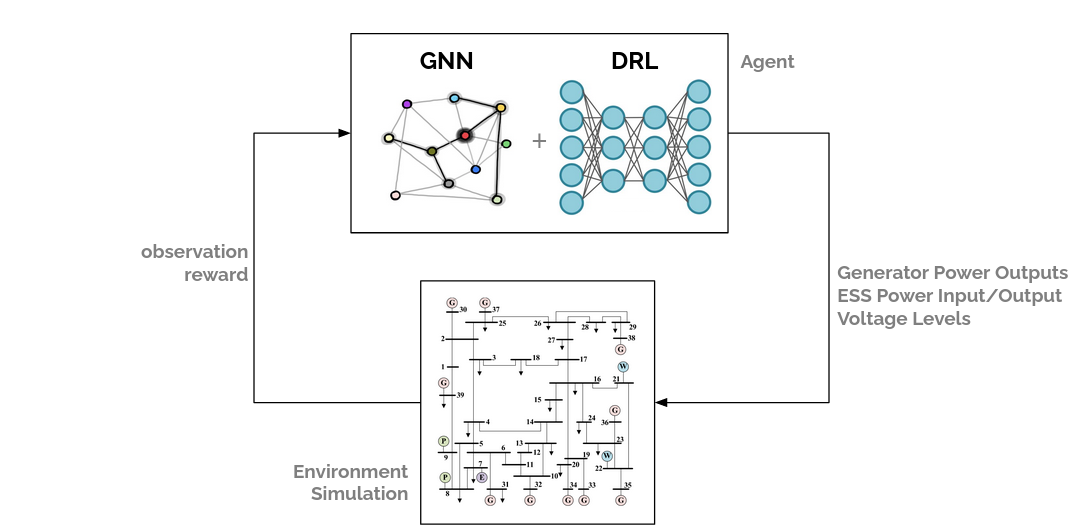
\includegraphics[width=0.85\linewidth]{./figures/arch.png}
	\caption{Solution Architecture}
	\label{fig:arch}
\end{figure}


To fulfil this, the agent adjusts the generator power output and voltage levels and manages the \ac{ESS} operation in real-time. \par
The solution is executed in the context of a power grid simulation that models the appropriate elements, properties, constraints and operating of the power distribution grid. This method is further described in the upcoming subsection \ref{sec:method}.

\section{Methodology} \label{sec:method}

\begin{comment}
	* Evaluative mehtods as subsection?
\end{comment}

Regarding the established methodology for enabling the implementation of the proposed solution, the \textit{grid2Op} framework \cite{rtefranceGrid2OpDocumentation} will be used for modelling the sequential decision-making process on simulated power distribution grid. \textit{grid2Op} is designed by RTE (\textit{Réseau de Transport d'Électricité}), the electricity transmission system operator of France, and is equipped with a variety of pre-defined scenarios used in coding competitions and based on real-world data \cite{rtefranceGrid2OpDocumentation}. This platform focuses on easing the job using the grid topology to control the power flows and also allowing for it to be reconfigured in real-time \cite{rtefranceGrid2OpDocumentation}. Additionally, enables to graphically plot the current observable state of the grid, as portrayed in figure \ref{fig:grid2op-graph}. Apart from graph topology, \textit{grid2op} also enables the manipulation of:

\begin{itemize}
\item the \textbf{voltages} by manipulating the set-point value of the generators;
\item the \textbf{active generation} by mapping the received observations to optimal sequences of dispatch actions \cite{rtefranceGrid2OpDocumentation}
\end{itemize}

This framework is compatible with the \textit{Gymnasium} framework \cite{faramafoundationGymnasiumDocumentation}, a widely used toolkit for developing \ac{RL} algorithms, which will also will be used in this work together with the Grid2Op simulation environment. 

\begin{figure}
	\centering
	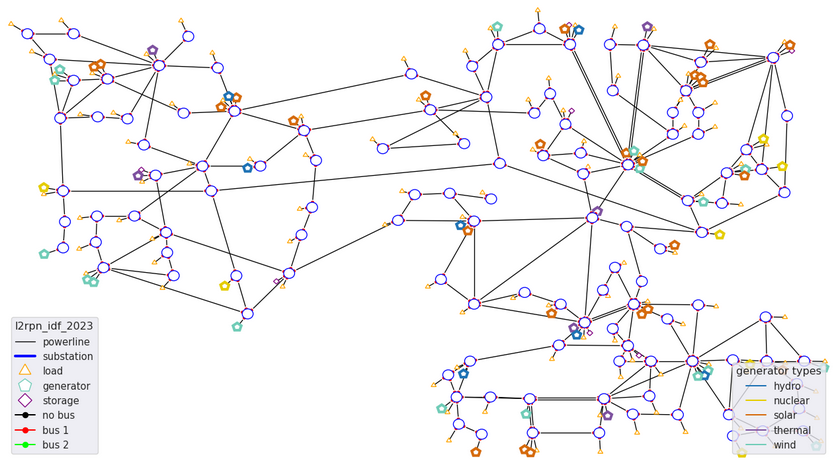
\includegraphics[width=0.85\linewidth]{./figures/grid2op-graph.png}
	\caption{Grid2Op \textit{l2rpn\_idf\_2023} 118-bus test case \cite{rtefranceGrid2OpDocumentation}}
	\label{fig:grid2op-graph}
\end{figure}

This platform focuses on describing the power distribution grids by modelling the following objects:
\begin{itemize}
	\item \textbf{Buses} are the fundamental objects of the power grid, representing nodes where power sources, loads and other elements are connected\cite{rtefranceGrid2OpDocumentation}.
	
	\item \textbf{Powerlines} represent edges in the power grid and connect the different buses together. They represent the physical transmission and distribution lines and allow power to flow from one part of the grid to another \cite{rtefranceGrid2OpDocumentation}.
	
	\item \textbf{Generators} are critical grid elements connected to buses whose main role is to produce power and maintain grid stability by balancing the energy supply and demand. They can be Conventional Thermal Generators, Wind Turbines or Photovoltaic Cells \cite{rtefranceGrid2OpDocumentation}.
	
	\item \textbf{Loads} consume power from the grid, simulating electricity use. They're also associated to an individual bus \cite{rtefranceGrid2OpDocumentation}.
	
	\item \textbf{Storage Units} can act as both consumers and producers. They're able to retain energy from the power grid when production surpasses demand for later injecting back power when convenient. Storage units are bound by a maximum energy storage capacity \cite{rtefranceGrid2OpDocumentation}.
\end{itemize}

\begin{table}[H] 
	\centering
	\caption{Test Case Sizes}
	\begin{tabular}{|P{2cm}|P{3.5cm}|P{3.5cm}|  }
		\hline
		 & \textbf{l2rpn\_icaps\_2021} & \textbf{l2rpn\_idf\_2023} \\
		\hline
		\textbf{Buses} & 36 & 118 \\
		\hline
		\textbf{Powerlines} & 59  & 186  \\
		\hline
		\textbf{Generators} & 22 & 62  \\
		\hline
		\textbf{Loads} & 37 & 99 \\
		\hline
	\end{tabular}
	\label{tab:test-case}
\end{table}

This work will use the pre-defined \textit{grid2op} \textit{l2rpn\_icaps\_2021} and \textit{l2rpn\_idf\_2023} test environments, a modified case studies based on the original IEEE 118-bus system test case \cite{christiePowerSystemsTesta} of 36 and 118 buses, respectively. The first test case is a subset of the original 118-bus system with 50 years worth of data divided into independent \footnote{non-consecutive} weekly scenarios, while in the second case the system was modified to accommodate the \textit{possible energy mix} of France in 2035, containing 16 years of data \cite{rtefranceGrid2OpDocumentation}. The scenarios document the loads and productions at each time step, the grid layout (for display purposes), generator and \ac{ESS} characteristics \cite{rtefranceGrid2OpDocumentation} for a weekly episode, the sizes of test cases can be further observed in table \ref{tab:test-case}. In addition, the test cases data will be modified to reflect the defined requirements of this work. \par
Beyond \textit{grid2op} to build and run the test cases and \textit{gymnasium} as the RL framework, this project will use \textit{PyTorch} \cite{pytorchPyTorch} with \textit{PyTorch Geometric} \cite{pygteamPyGPytorch_geometric} library for developing the \ac{GNN} because of its extensive list of available implemented models. The different combinations of algorithms will be applied to a set of modified scenarios that fulfil the settled requirements. For Deep Reinforcement Learning algorithms, solutions with plain \ac{SAC}, \ac{DDPG} and \ac{PPO} approaches and combined with the \ac{GCN}, \ac{GAT} and \ac{GIN} architectures.  \par
Concerning result analysis, it's also important to point out the use of quantitative methods for evaluating the different implemented models, a topic that is further explored in the following section \ref{sec:eval-methods}.


\subsection{Evaluative Methods} \label{sec:eval-methods}

\begin{comment}
	* Sample Efficiency
	* Other methods
\end{comment}


The solution described in the previous subsections \ref{sec:arch} and \ref{sec:method} clearly involves intricate operational mechanisms, something that calls for a sophisticated evaluative process. Furthermore, given the comparative nature of this dissertation the evaluation and analysis methods will be key factors in studying and confronting the different combinations of \acp{GNN} and \ac{DRL}, as well as possible improvements in the integration of these techniques.
In this manner, we define the four dimensions for evaluating and analysing the different \ac{GRL} models:

\begin{description}
	\item[Learning efficiency] This dimension assesses how effectively the models learn and improve their decision-making process over time. It involves evaluating how quickly they converge to optimal or near-optimal dispatch strategies through the convergence rate. 
	
	\item[Computational Efficiency] It's crucial that the solution is able to perform well on real-time execution. In this context, not only it's important to assess the solution's decision computation performance but also to measure the time necessary for the model offline training, as well as the observed CPU/GPU resource utilization.
	
	\item[Dispatch Efficiency] The performance of the \ac{GRL} model in managing power distribution from the various generators will be mainly measured by the average operating cost (in \textit{Euros}) derived from the agent's sequence. Furthermore, other system behaviours will be analysed such as Renewable Energy Source Penetration, through the average ratio of maximum power and real power output, and \ac{ESS} utilization, through the average energy stored.
	
	\item[Scalability and Adaptation]  The solution will be applied to scenarios of several sizes for analysing its scalability. Furthermore, we will induce variations in the simulation scenarios to test the model's ability to handle topology changes.
\end{description}

\section{Work Plan} \label{sec:work-plan}


In order to make this project possible, we propose a 40-week work plan divided into four stages, whose start was in the last week of September 2023 and expected conclusion is scheduled for the last week of June 2024, observable in figure \ref{fig:gantt-chart}. 
The first stage, ranging from the first week of the plan to the delivery of this report, encompasses the \textbf{dissertation preparation} phase. This stage mainly addressed the initial knowledge acquisition necessary to understand this work's context and gather a basic grasp on the concepts and topics it addresses, namely:
\begin{itemize}
	 \item Reinforcement Learning
	\item Graph Theory
	\item Graph Representation Learning
	\item Graph Reinforcement Learning
	\item Graph Neural Networks
	\item Smart Grids Services
\end{itemize}
This process is followed by the analysis of existing research and approaches in \ac{GRL} and Smart Grid technologies which spans till the first week of January 2024, documented in chapter \ref{chap:literature-review}. Lastly, the preparation phase is also compromised of the PDIS report write-up until its delivery in the first week of February 2024, marking the end of this phase. \par
The preparation phase is followed by the \textbf{Development} phase. This stage encompasses all activities related to the system implementation, from the preparation of the simulation environment to the model training and calibration. The development phase spans from the first week of February 2024 to the second-to-last week of April 2024. \par
Next, the \textbf{Evaluation \& Analysis} stage is set, compromising the time frame where the various implemented models will be evaluated in the context of the previously mentioned dimensions and the evaluation results will be analysed. \par
Lastly, the \textbf{Dissertation} write-up and subsequent revision work will be performed, compromised of the write-up, proofreading and correction tasks and ranging from the end of the evaluation and analysis phase in the last week of April 2024 until the last week of the plan.


\begin{sidewaysfigure}
	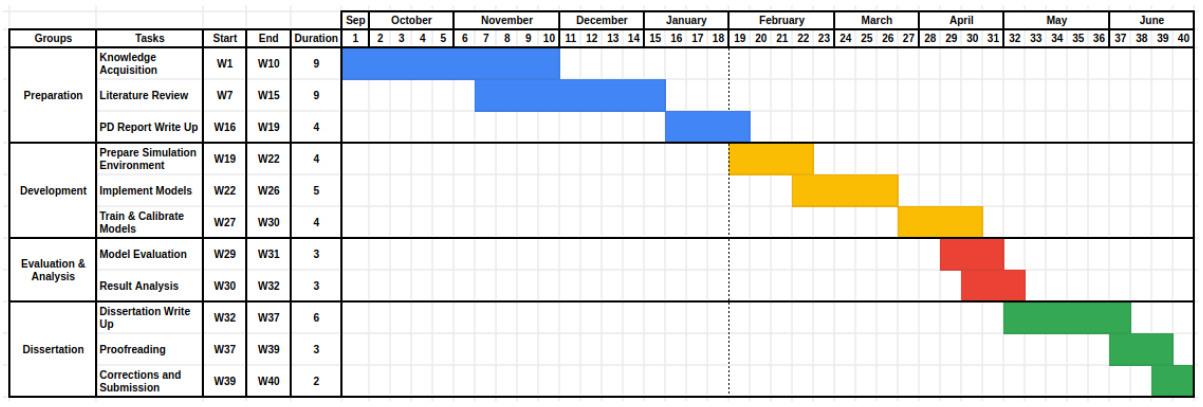
\includegraphics[width=1.0\linewidth]{./figures/gantt-chart.png}
	\caption{Project Work Plan}
	\label{fig:gantt-chart}
\end{sidewaysfigure}

